This chapter serves as an overview of select existing online reservation systems and can be taken as a form of market research for the booking system to be created.

The overview is meant to be qualitative rather than quantitative, focusing on the exploration of features provided by a select few systems and the user experience while using those systems. The systems chosen for the overview are Acuity Scheduling\footnote{Acuity Scheduling (\url
{https://www.acuityscheduling.com})}, Reservio\footnote{Reservio (\url
{https://www.reservio.com})}, Square Appointments\footnote{Square Appointments (\url
{https://squareup.com/us/en/appointments})}, and Wix\footnote{Wix (\url
{https://www.wix.com})}.

The criteria used to choose the systems for the overview are the following:
\begin{itemize}
    \item \textbf{Popularity} --- The system must be popular with the public. Without an extensive quantitative survey, this is a difficult criterion to evaluate. As a rough estimate, the system's ranking in the Google search results for the queries \enquote{online reservation system,} \enquote{online booking system,} and \enquote{online scheduling system} was used. If the systems appeared on the first couple of pages of the results, they were considered popular enough. Some flaws of this approach are, for instance, results personalization based on geographic location, as well as search engine optimization (SEO) techniques used by the systems. Similarly, different systems could have been discovered by using other search queries and search engines. However, despite the flaws of this approach, it still seemed to yield good enough results.
    \item \textbf{Localization} --- The system must have English localization.
    \item \textbf{Price} --- The system must offer a free version of its service (at least as a limited-time trial). Additionally, it must not require payment information to sign up for the free version.
\end{itemize}

\section{Acuity Scheduling}
\label{part:acuity_scheduling}

Acuity Scheduling~\cite{acuity} describes itself as \enquote{an online appointment-booking tool} that \enquote{is great for any business that needs clients to book appointments for services in advance.} It also says that \enquote{businesses including yoga studios, massage therapists, acupuncture, life coaches, photographers, hair and nail salons use Acuity with great success,} but that it \enquote{is not a great fit for businesses that want to book appointments that last more than a day, like car rentals, vacation rentals, or hotels.} Acuity Scheduling is a subsidiary of Squarespace -- a company that primarily focuses on providing a website-building service (for some time after Squarespace acquired Acuity, the scheduling product was rebranded to Squarespace Scheduling, but that change has since been reverted).

The website offers a free limited-time trial, after which it cannot be used without paying for one of its tiered plans. After first singing up for a business account, the user is asked for the name of their business and the name of an Acuity Scheduling subdomain that the service will create for the booking website of the business (this is optional, and if not provided, the website will be available under a shared subdomain and a URL query parameter with a generated identifier).

The user then creates their first appointment type by filling out the name of the appointment, its duration, whether it is a one-on-one appointment or a group appointment, and optionally, its price. If the user has selected the group appointment type, they must set the number of open slots per class as well.

Moreover, the user sets up the availability of the created appointment type by selecting a date and a time, whether or not it is a recurring event, and, if it is, the frequency of the recurrence (such as every Monday, every other Tuesday, the first Wednesday of each month, or daily), and the number of recurrences.

Lastly, the user can optionally connect third-party payment processors (Stripe, Square, and PayPal) for collecting deposits or full payments for the appointment bookings. Long-term subscriptions are also supported. The service claims~\cite{acuity} that it does not take any commission on the payments and that the only fees are those charged by the payment processor.

After the business user completes the sign-up process, customers can access a booking website that is created for the business. Upon accessing the website, customers see the business information (with only the sign-up completed, that is just the business name), followed by a list of appointments to choose from, with each appointment featuring its name, time and date, duration, and a sign-up button. If the business user selected the group appointment type, there is also a quantity field above the appointment list and the number of free spots available under each appointment's sign-up button. Signing up for a selected appointment is followed by filling out personal information (a full name, an email address, and optionally a phone number). If there was no payment required, the customer completes the booking and receives an email with the details of their booking, a link to reschedule or cancel the appointment, and links to add the appointment to their calendar. The booking page can be seen in the figure~\ref{fig:acuity_scheduling}. The customer can use an account to manage their booked appointments, but it is purely optional, and they can still manage their bookings through the email links. There is also no way for the business to limit their appointments to only signed-in customers (the business can, however, ban clients by their email address).

The scheduling functionality can be integrated into any website built with Squarespace (which can then use a custom domain). There are also simple booking components that can be embedded into another website, in addition to the option to embed a booking page iframe. The booking website can be customized by choosing between a couple of predefined layouts and can also use custom CSS. The platform also features webhooks and an extensive application programming interface (API), which can be used to integrate it with other applications.

Business users can see all their appointments in a calendar overview, as well as all their clients. Under each appointment in the calendar, the user can see all signed-up customers, reschedule or cancel their bookings (when the business user does this, the affected customer can be notified by email, but there is also an option not to send this notification), and add private notes and tags for each customer. The user can manually add new attendees to each appointment (which can be useful, for example, when a customer wants to create a booking over the phone, but the business wants to have everything tracked in the booking system). There is also an option to send an email to all attendees of a selected appointment, in addition to SMS reminders. The business user can be notified of new activity by email as well, and they can synchronize their calendar with other popular calendar applications.

Appointment types can be further customized by adding a color and a picture. Users can make appointments private, in which case they are not visible to the public and can only be accessed through a direct link. There is an option to require clients to sign up for every recurrence of a recurring appointment and an option to disallow clients from booking multiple spots. Appointment types can also have a form added for the customers to fill out before booking an appointment. The form can consist of questions with answers of several different types, including a text field, a drop-down list, a checkbox, and even a file upload. The business information shown on the booking website can also be customized a bit further by, for instance, adding a logo, filling out rich content instructions for the customers, and changing to one of a few different languages.

Other features available include CSV import and export of clients and appointments, setting limits on how long before an appointment it can be canceled or rescheduled, and adding Google Analytics to the booking website. A business account may be used by multiple users with separate login credentials and role-based permissions.

\begin{figure}
    \centering
    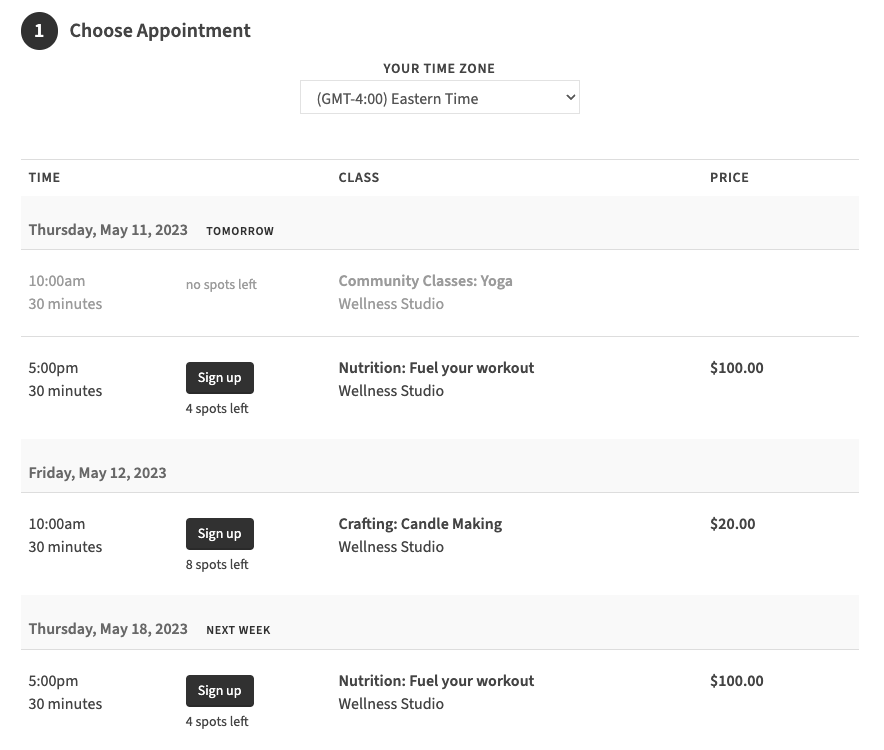
\includegraphics[width=1.0\textwidth]{content/existing_reservation_systems/acuity_scheduling.png}
    \caption[Acuity Scheduling]{Acuity Scheduling~\cite{acuity}}
    \label{fig:acuity_scheduling}
\end{figure}


\section{Reservio}
\label{part:reservio}

On the front page of its website~\cite{reservio}, Reservio describes itself as a \enquote{free online scheduling software for gyms, fitness centers, hair studios, barbershops, nail salons, car repair, medical services, teachers and educational institutions, group events, and more.}

When a user first signs up for a business account, they are asked to provide the following information:
\begin{itemize}
    \item the name of their business;
    % https://www.grammarly.com/blog/comma-between-correlative-conjunction-sets/
    \item the type of their business, which can be either \enquote{Single appointments} (described as \enquote{the client books a service or an appointment at a specific time}) or \enquote{Group events} (described as \enquote{host multiple clients at the same event, lecture or course}); to change this business type later on, one must contact customer support;
    \item opening hours, which \enquote{determine the exact range of when your clients can make bookings} and can also be customized per employee;
    \item the physical address of their business;
    \item optionally the contact phone number of their business;
    \item and optionally other information about their business -- a website, a slogan, a description, and additional information about the physical address.
\end{itemize}

Users are also asked to add the services they would like to provide to their clients. Each service must have a name and a duration, and can optionally have a description, a price, a color (to visually differentiate it from other provided services), and an additional question to ask the customers (which can also serve as an input for a voucher code).

Lastly, users can also add staff members of the business who provide the previously added services, each with a name, a checklist of the services they provide, and optionally a short biography.

After the user completes the sign-up process, customers can access a booking website that is created for the business on a Reservio subdomain. When a customer accesses the booking website, they immediately see all the information about the business that was provided during the sign up. They then select a service for booking, a staff member (or \enquote{anyone available}), a date from a calendar picker, and a free time slot for the selected date. The customer can complete their booking either as a guest or by creating a Reservio account (or logging into an existing account). If the customer chooses to create an account, they can also see their booking history and cancel their bookings (in the settings, a business can set how long before the event can the bookings be canceled). The business user can also restrict in the settings who can create bookings to for example only existing clients or only clients with an account. As the last step of the booking process, the customer can answer the additional question that was added by the business, and they may also add a note. Afterwards, the customer is sent an email with the details of their booking.

For group events, the process is very similar, with the business user additionally specifying the capacity of an event. The customers can then book multiple spots for an event, as long as there is sufficient space available. Group events can also be marked as private by the business user, in which case they are not visible to the public and can only be accessed through a direct link.

The booking page iframe or simple booking components can also be embedded into another website. The booking website can be set as indexable by search engines and can use a custom domain instead of the Reservio subdomain (for premium accounts only). The layout and theme of the booking website can be somewhat customized as well, though most of the customizations are limited to premium accounts. There is an extensive API which can be used to integrate Reservio with other applications.

Business users can see their existing bookings in a calendar (also available as per staff member and per service views) which can be seen in the figure~\ref{fig:reservio}, as well as an overview of their clients. Premium users can have their calendar be synchronized with other popular calendar applications. Users can edit and cancel the existing bookings, as well as manually add new bookings and clients. Unreliable clients can be blocked and there is a CSV file import of clients as well. The amount of bookings a business can have is limited by different premium subscription plans.

Other available features include the ability to receive email and SMS notifications about new and canceled bookings (though SMS is limited to premium accounts), client reminders a set number of days or hours before a booked event, the option to limit the time of user data retention, and adding analytics to the booking website (such as Google Analytics and Meta Pixel; limited to premium accounts). Businesses can opt in to have their profile listed in a service marketplace (which customers can access through a separate application). One business account may be used by more staff members with separate login credentials and role-based permissions.

The platform also features online payments (which can be set as mandatory or optional), for which it takes a commission: This feature includes the handling of refunds when a customer cancels their booking and the possibility of long term memberships. However, according to Reservio~\cite{reservio}, this feature is currently only available in the Czech Republic where the company originates and for security reasons it does not work when a custom domain is set up for the booking website.

\begin{figure}
    \centering
    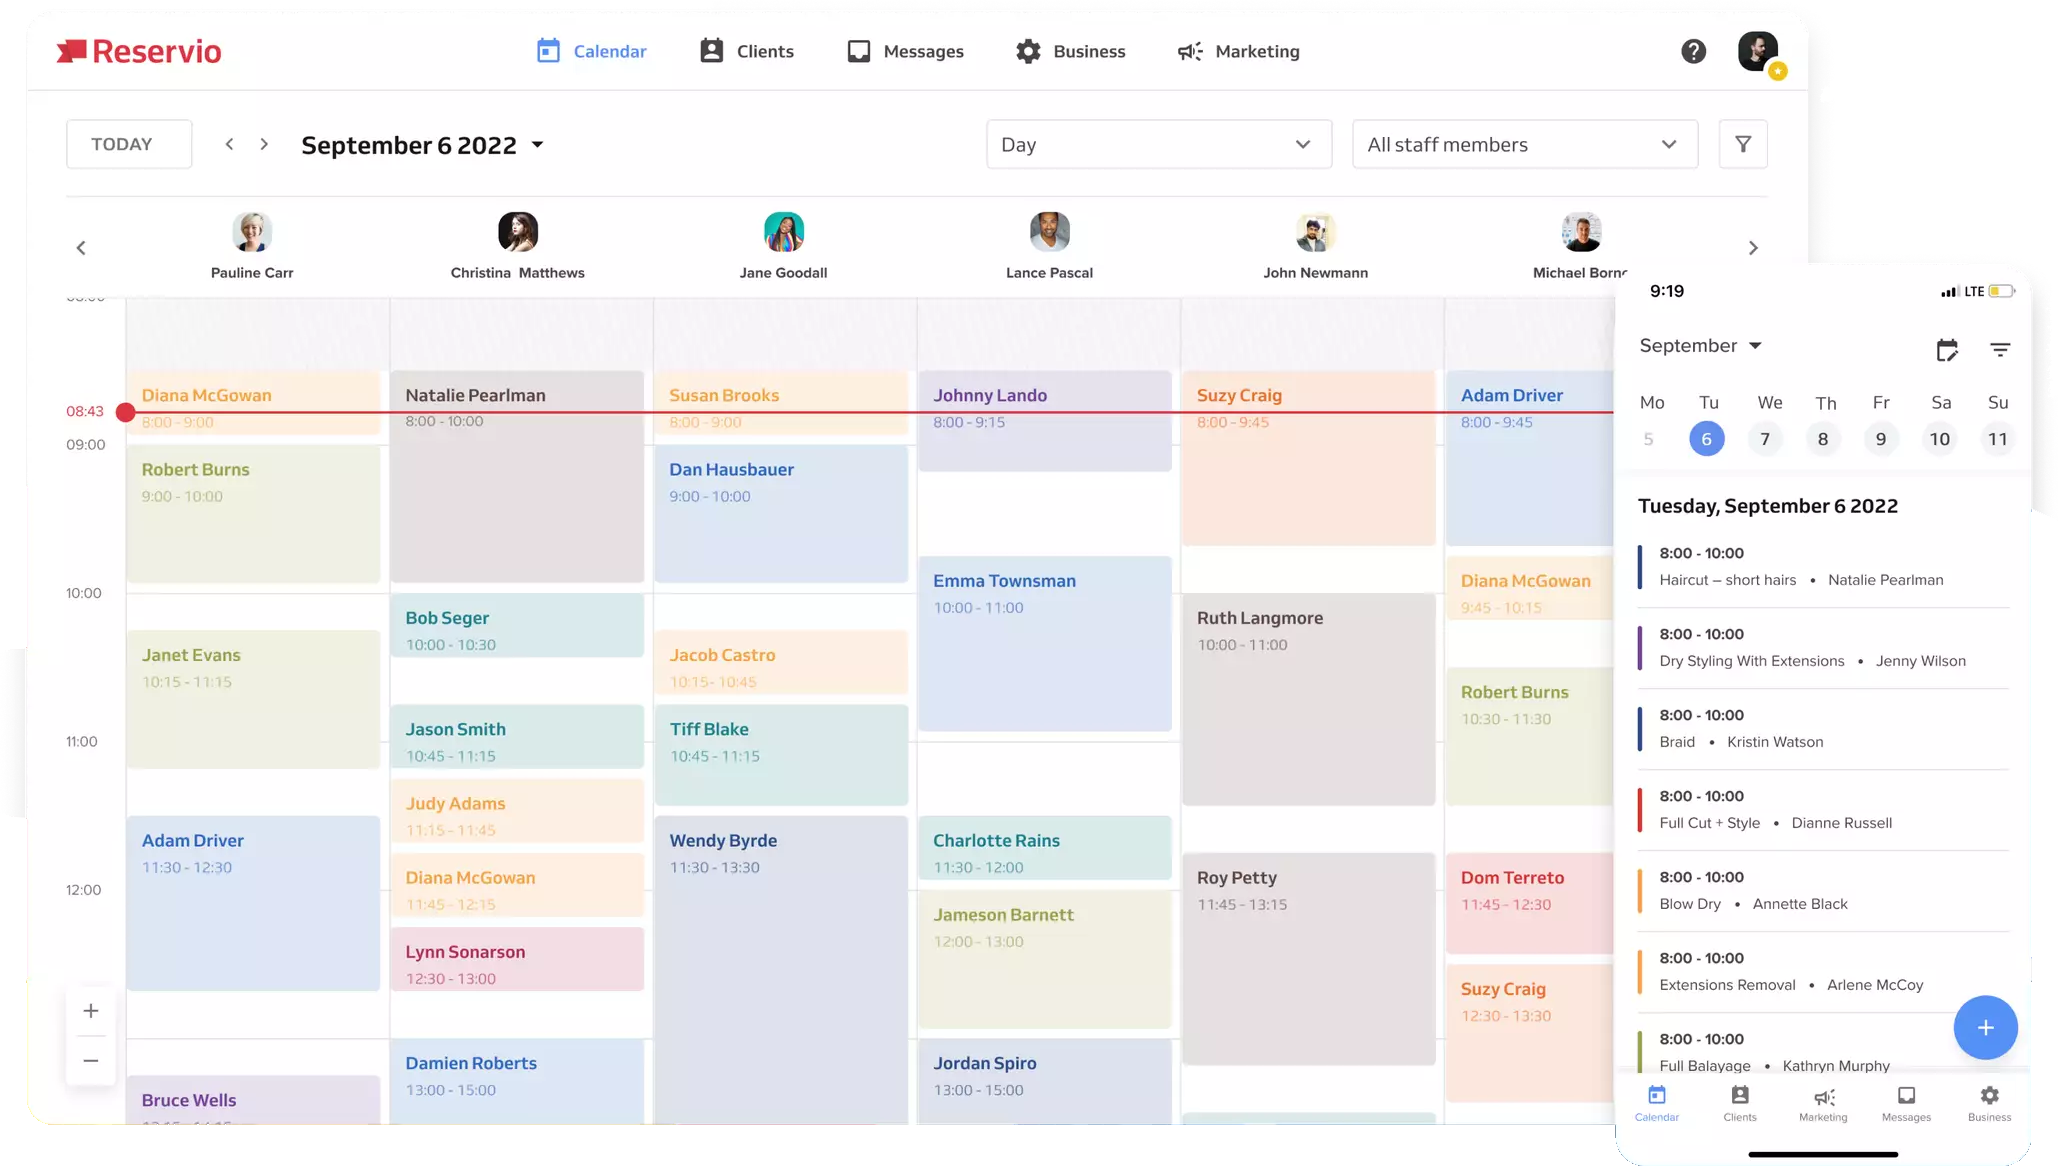
\includegraphics[width=1.0\textwidth]{content/existing_reservation_systems/reservio.png}
    \caption[Reservio]{Reservio~\cite{reservio}}
    \label{fig:reservio}
\end{figure}


\section{Square Appointments}
\label{part:square_appointments}

Square Appointments~\cite{square} is a product by the company Square (not to be confused with Squarespace, which is a different company), which primarily focuses on providing financial services to businesses (some other reservation systems mentioned in this overview even offer Square as a payment processor). Square Appointments~\cite{square} describes itself as \enquote{the all-in-one point of sale for
booking, payments, and more.}

After first signing up for a business account, the service asks the user to provide some basic information: their personal name, business name, business phone number, time zone, and the type of the business. This information is later shown to the customers on an online booking site, if the business chooses to have one.

Square also asks for the number of staff members, business locations, and optionally services offered. The user also must fill out their estimated monthly revenue and optionally can input the average price per client. Then the user selects which features they are interested in, which can be any of the following: customizable online booking site, selling products, accepting payments, prepayment and no-show protection, and automated reminders and confirmations. For the purposes of this overview, the customizable online booking site, as well as the automated reminders/confirmations were chosen.

Square Appointments offers a feature-limited free plan (which is also limited to a single business location), as well as a limited-time trial of their lowest tier paid plan. The trial was used for this evaluation.

In the administrative dashboard, the user can edit their business location details, including its physical address, contact information, and social media links. They can add a short description of their business, a logo, and business hours.

The user then creates services that they offer, by filling out the service name, description, price, and duration. The service can have an image attached to it and its business location specified (when the business has multiple locations). A cancellation fee can be set up, and there can be extra time added to be blocked off after the service is done (for example for cleaning). The service can be categorized and team members can be assigned to it.

Finally, the user enables online bookings and can set up a customizable Square Online website with booking functionality built in. This website is published to a Square provided subdomain, and a custom domain can be set up as well (with a premium account). The booking functionality can also be embedded into an existing website using a button component or an iframe.

When a customer visits the booking website, they can see basic information about the business (such as its name and phone number), the services they provide, their staff, and locations including the opening hours. To create a booking, the customer selects the services they want to book, the date from a calendar picker, one of the available time slots from a list, then they fill out their personal information (phone number, email address, and full name) and optionally any note for the business. If the business sets up multiple staff members for a service, the customer may select a preferred staff member as well.

Upon booking, Square automatically creates an account for the customer, which they can sign in using the provided phone number (this cannot be skipped). The booking can be added to their personal calendar by one of several popular calendar services. The customer can reschedule or cancel their booking. The customer also receives an email with the booking details.

The business user can view their calendar, which includes the customers' bookings. They can view each booking's details, edit and cancel the booking. Bookings can be added manually as well. The business calendar can be synchronized with Google Calendar. The business calendar can be seen in the figure~\ref{fig:square_appointments}.

In the settings, the business user can also choose to require manually accepting all bookings. Time limits for scheduling can be set as well. The list of staff can be removed from the booking website. An interesting feature is the so-called \enquote{Fake-it Filter} which lets the business \enquote{remove some of their availability to give the appearance that their business is busier.} Email and SMS reminders can be set up to be sent to the customers a given time before their appointment. There is no option to add a form to the booking process, but there is an option to create a form to send clients afterwards.

Other features include multiple team members using the business account with different permissions, a waiting list that automatically notifies clients of new availability, and an API. For some types of businesses, there is also a marketplace application from Square, where businesses can set up a profile for clients to discover. As square as a platform is primarily focused on offering financial services, there is a lot of detailed features related to this, including subscriptions management, thorough receipt customization, or various options regarding taxes, fees, and money transfers. Square also offers hardware for on location payments.

\begin{figure}
    \centering
    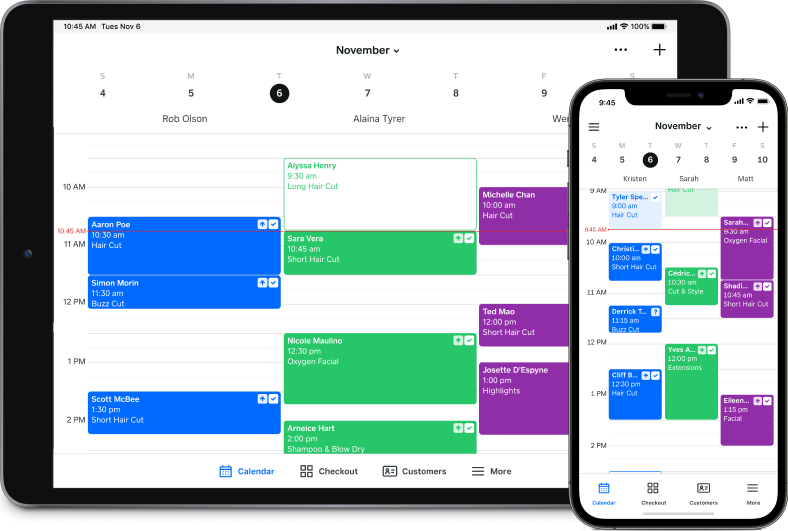
\includegraphics[width=1.0\textwidth]{content/existing_reservation_systems/square_appointments.png}
    \caption[Square Appointments]{Square Appointments~\cite{square}}
    \label{fig:square_appointments}
\end{figure}


\section{Wix}
\label{part:wix}

Wix~\cite{wix}, similarly to Squarespace (mentioned in a prior section of this overview), mainly offers a website building service which enables users to create their own websites using the Wix Website Builder UI. When building a website, users can make use of the so-called Wix Apps found in the Wix App Market. These can be thought of as plugins/extensions that the user can use to add functionality to their website or to the administrative dashboard. Wix Apps can be either official ones developed by Wix, or third-party ones (Wix provides an extensive API and even options to monetize the Apps published in the Wix App Market).

Wix offers three official Wix Apps which can in various ways be used to add reservation functionality to a Wix website: Wix Bookings, Wix Events, and Wix Restaurants. Wix Bookings seems to be meant for businesses offering frequently occurring appointments or classes. Wix Events appears more suited for those who organize events that only happen a few times or infrequently (Wix~\cite{wix} lists \enquote{planning a wedding, hosting a convention, or selling tickets to a show} as examples). Wix Restaurants, as the name suggests, focuses purely on restaurant businesses, enabling them to for example showcase their menu, receive orders, but also to set up online reservations.

This overview focuses on Wix Events, which are available as part of Wix's free plan (with some limitations), and briefly on Wix Bookings, which do not work with the website as part of the free plan, but do at least let users set up the administrative section.

After first signing up for an account, Wix asks the user a few questions about the purpose of their website to be built. Based on these answers it customizes the UI a bit, including adding suitable Wix Apps. When choosing the \enquote{Book Event} option as the primary focus of the website, the user is directed into the setup of the already installed Wix Events. They create their first event by entering the following:
\begin{itemize}
    \item the name of the event,
    \item the type of the event -- either a \enquote{Ticketed event} with options for pricing and availability or a \enquote{Registration only} event meant to collect confirmations of an invitation (RSVPs),
    \item the starting time and date of the event,
    \item optionally the ending time and date of the event,
    \item whether it is a recurring event (this lets the user add multiple dates/times for the event, but there does not appear to be an option to do this automatically),
    \item and optionally the location of the event (which can be a physical address or online).
\end{itemize}

The user can then add various tools to their website. These tools include for example a seating map which can \enquote{let guests choose their seats} or email marketing which can send invitations.

Lastly, the user can set up a custom domain to use for their website (though this is only available with a paid plan; otherwise the service provides a free Wix subdomain), design their website, and optionally optimize the website's SEO. If the user selected the \textit{Ticketed} event type, they also need to create ticket types for the created event to be bookable.

For designing the website, there are ready-made layouts which can be customized to a great extent, since that is Wix's primary focus. The user can also let the service use artificial intelligence (AI) to generate the website layout for them. Since this overview's goal is not to evaluate website builders, the AI option was chosen to save time. The resulting layout appeared fairly usable, though it seemed to have issues adjusting to different window sizes.

In the event details, the user can additionally provide a description and an image for the event. Events can be grouped into categories. Creating a ticket asks for the name of the ticket, optionally its description, the number of tickets available, a pricing method, and a window of time when the ticket is available for purchase. Tickets can be limited to a maximum amount per single order.

The pricing method can be fixed to a certain amount, split into different categories (e.g. child, adult), \enquote{pay what you want,} and free. Wix lets users connect third-party payment processors to collect these payments (such as PayPal and Stripe, but the availability of the payment processors depends on the user's country), and it charges a service fee (which is added on top of the payment processor's fee).

Events can have forms attached, which can include fields of multiple different data types. With the seating map tool, the user can create a detailed map of the seats and areas available at the event venue. They can then assign the available tickets to specific seats or areas. This seating map from the customer's perspective can be seen in the figure~\ref{fig:wix_seating_map}.

When all of this is set up, the user can publish the event on their website. Customers who access the website then navigate the event, see its details (such as the name, the time and date, and the location) and available tickets. If the window, during which tickets are up for sale, is open, they choose the ticket to buy by selecting the seat or admission area from the map (or, if no seating map was added, just choose which type of ticket to buy and its quantity), fill out any form the business user attached to the event, and check out. The customer can then download their tickets as a PDF document and add the event to their personal calendar. They also receive an email with the details of their booking.

The tickets that a customer receives include a QR code in them, which can then be scanned on location by the event organizer using a special-purpose mobile app from Wix. It does not appear that a customer can reschedule or cancel their booking, though the business user can do this for them (as well as cancel the event completely) through an overview of their orders and guests, though according to Wix~\cite{wix}, they will need to handle any refunds themselves. The business user can also add guests manually and later on manually check in any guest.

The Wix Bookings App adds a section with a booking calendar to the administrative dashboard. The user can add a service they would like to provide to their customers, which can be either an appointment (described as \enquote{a private session that can be booked according to availability}), a class (described as \enquote{a group session that can recur} where \enquote{clients book any session they want to join}), or a course (described as \enquote{a set of group sessions} where \enquote{clients book them all up front}).

In addition to providing some basic details about the service, the user can add pricing or a long-term membership plan, as well as staff members who provide the service. A booking form can also be attached. Unlike with Wix Events, the booking can be canceled or rescheduled by the customers, since there are options to disable this and limit the period of time before the booking when such changes can be made. Additionally, there is an option to require manually accepting all bookings.

The business user also sets up their opening hours, so that the service can offer recurring classes during these times (unlike with Wix Events, where recurring events had to have their times and dates added manually). A useful feature is also the option to schedule the appointment time slots either based on the service duration or every fixed amount of time. Booking reminders through email and SMS, calendar synchronization, and waiting lists are available as well. An example of a Wix website with the Wix Bookings functionality can be seen in the figure~\ref{fig:wix_bookings}.

Other features of the platform include built-in website analytics, multiple staff members managing a single account with role-based permissions, business website localization, CSV export of orders, and a full-featured API.

\begin{figure}
    \centering
    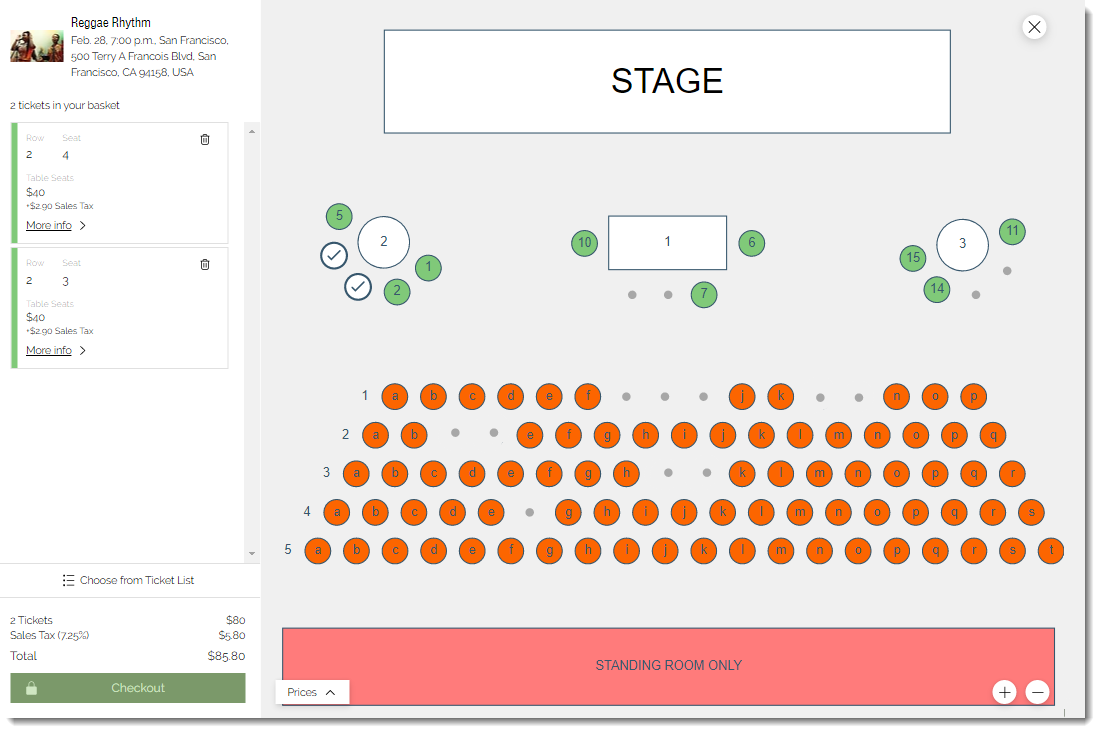
\includegraphics[width=1.0\textwidth]{content/existing_reservation_systems/wix_seating_map.png}
    \caption[Wix Events]{Wix Events~\cite{wix}}
    \label{fig:wix_seating_map}
\end{figure}

\begin{figure}
    \centering
    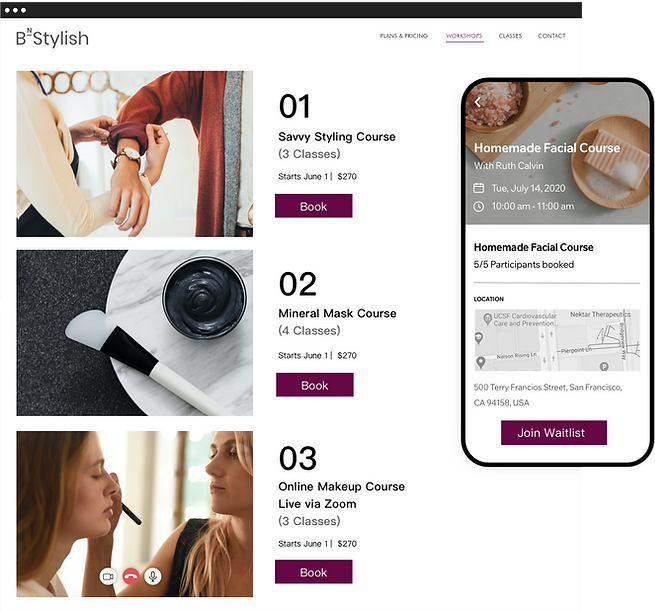
\includegraphics[width=1.0\textwidth]{content/existing_reservation_systems/wix_bookings.png}
    \caption[Wix Bookings]{Wix Bookings~\cite{wix}}
    \label{fig:wix_bookings}
\end{figure}


\section{Summary}
\label{part:existing_reservation_systems_summary}

To summarize this overview, among the four online reservation systems included in the overview -- Acuity Scheduling, Reservio, Square Appointments, and Wix -- there were many similarities and common features.

One of the similarities was the overall process of setting up a business account, filling out basic information about the business and setting up certain services, classes, or events for the clients to book. After this, the system would let the users create a booking website under the subdomain of the service or under a custom domain (which was always a premium feature). Customers could then access the website, view the information about the business, the services or events provided, and create a booking.

All systems also featured some options to accept payments, in addition to sending out emails with booking details and reminders. There was always some possibility to embed components or iframes with booking functionality to other websites, and an API for developers to integrate the system with other software (the API was always platform specific though). Calendar synchronization and multi-user accounts (with adjustable permissions) were also common features.

The main differences (excluding pricing strategies and the UI) seemed to be the ability to add forms for users to fill out during booking (present in Acuity Scheduling and in Wix's solutions), the ability to create a custom venue map with seating and areas sold under different ticket types (present in Wix Events).

Those platforms that focus on building websites (Wix and -- the owner of Acuity Scheduling -- Squarespace) offer more features for extensive booking website customization. On the other hand, Square Appointments from Square who focuses on financial services, offers the most features for payment processing, customer subscriptions, and financial reporting. Finally, Reservio seemed to offer subjectively the simplest business account setup and UI.

